%!TEX root = thesis.tex
\chapter{Infinite Projected Entangled Simplex State}
\label{chapter:ipess}
\section{Simplex-solid State}
\label{solidstate}
The simplex-solid state of an SU(N) quantum anti-ferromagnet was derived by Arovas \cite{} and the most significant conclusion is that any simplex states could be described by a natural generalization of the AKLT \cite{} valence bond solid state, which means that the bond signlets of the AKLT could be extended to N-site simplices.

The concept of simplex-solid states ansatz were introduce by Xie et al \cite{}. The tensor-network representation of simplex states is called projected entangled simplex state (PESS) which is also considered as an extension of PEPS \cite{} obeying the area law of entanglement entropy and characterizing any states if the dimension of the virtual bonds are large enough. The difference from the PEPS is that the entanglement among the virtual particles is described by entangled simplex tensors which depend on the structure of PESS. For example, in Fig. \ref{fig411}(b) there are three virtual particles within the simplex state, so the entangled simplex tensor $S_{mnl}$ is a rank-3 tensor.

\begin{figure}[ht]
	\centering
	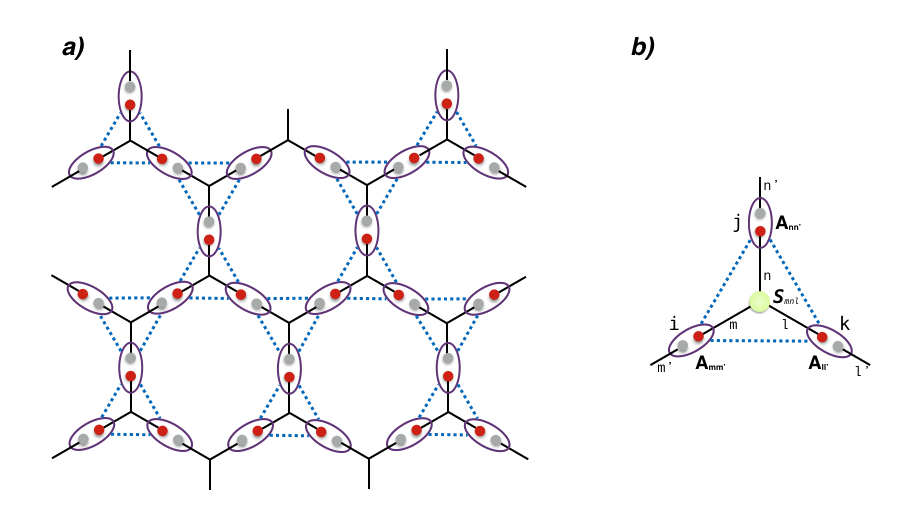
\includegraphics[width=0.80\textwidth]{figures/fig411.png}
	\caption[The picture of the main idea of itebd.]{The red and blue tensor denotes on \textit{odd} and \textit{even} sites. The yellow one are time evolution operators $e^{-\tau H_{k,k+1}}$, $e^{-\tau H_{k+1,k}}$}
	\label{fig411}
\end{figure}

For illustrating how to write down the formulation of the PESS wave function, we begin from a simple system, the spin-2 simplex state on an infinite Kagome lattice \cite{}. See Fig. \ref{fig411}(a) each physical $S=2$ states on the lattices could be treated as a symmetric superposition of two virtual $S=1$ spins. According to the theory of AKLT, each neighbor simplices (triangles) share a single site symmetrically which also means that the $S=1$ spins could be assigned to one of the simplices (vertex-sharing). Hence, there are three $S=1$ spins in each simplex states. From the features of the $SU(2)$ group, the decomposition of the direct-product of three integer spins is written as, 
\begin{align}
	\label{su2}
	n \otimes n \otimes n = [a_0 \times 0] \oplus \dots \oplus [a_k \times k] \oplus \dots \oplus [a_{3n} \times 3n] \\
	a_k = \begin{cases}
		2k + 1 & \text{, $k \leq n$} \\
		3n + 1 - k & \text{, $k > n$} 
	\end{cases}
	\quad \text{, } k = 0, 1, \dots , 3n ,
\end{align}
where $a_k$ is a constant and $k$ express the $k$th irreducible representation. Now that we can write down the product of the spins in the simplex as,  
\begin{align}
	\label{111}
	\barbelow{1} \otimes \barbelow{1} \otimes \barbelow{1} = \barbelow{0} \oplus \left( 3 \times \barbelow{1} \right) \oplus \left( 2 \times \barbelow{2} \right) \oplus \barbelow{3},
\end{align}
and show that there is an unique spin-singlet state. The result encourage us to define a virtual singlet on simplex,
\begin{align}
	\Ket{\psi_{\alpha}} = \frac{1}{\sqrt{6}} \sum_{\left\{ s_i s_j s_k\right\}}{S^{\alpha}_{s_i s_j s_k}\Ket{s_i, s_j, s_k}},
\end{align}
where $s_i,s_j,s_k$ are $S=1$ virtual spins located at site $i,j$ and $k$ containing in the simplex $\alpha$ and $S^{\alpha}_{s_i s_j s_k}$ is the Levi-Civita antisymmetric tensor $\varepsilon_{ijk}$ [Fig. \ref{fig411}(b)]. For mapping the two virtual $S=1$ spins to the spin-2 subspace, we defined the projection operator $P_i$ on each site,
\begin{align}
	P = \sum_{s_i,s^{\prime}_{i}}\sum_{\sigma_i}{A^{\sigma_i}_{s_i,s_i^{\prime}}\Ket{\sigma_i}\Bra{s_i,s_i^{\prime}}}
\end{align}
where $\Ket{\sigma_i}$ is a basis of the $S=2$ spin at site $i$. $A^{\sigma_i}_{s_i,s_i^{\prime}}$ is a projected matrix whose components are filled by the Clebsch-Gordan coefficients,
\[
	\begin{aligned}
		&A_{11}^2 = A_{33}^{-2} = 1, \\
		&A_{12}^1 = A_{21}^{1} = A_{23}^{-1} = A_{32}^{-1} = \frac{1}{\sqrt{2}}, \\
		&A_{13}^0 = A_{31}^{0} = \frac{1}{\sqrt{6}}, \\
		&A_{22}^0 = \frac{2}{\sqrt{6}},
	\end{aligned}
\]
Now that we can write down the wave function of the simplex-solid state,
\begin{align}
	\Ket{\Phi} &= \bigoplus_i P_i \prod_{\alpha}{\Ket{\psi_{\alpha}}} \\
	&= \Tr \left( \dots S_{s_i s_j s_k}^{\alpha} A^{\sigma_i}_{s_i,s_i^{\prime}} A^{\sigma_j}_{s_j,s_j^{\prime}} A^{\sigma_k}_{s_k,s_k^{\prime}} \dots \right) \Ket{\dots \sigma_i \sigma_j \sigma_k \dots}.
\end{align}
and apply the tensor-network representation to descrbe it, see in Fig. \ref{fig411}(b).
This structure could be extended to any higher integer spins. In conlusion, a physical $S=2n$ (even-integer) spin is considered as a symmetric superposition of two virtual $S=n$ spins and a $S=2n-1$ (odd-integer) one is regarded as a symmetric superposition of a virtual $S=n-1$ spin and a virtual $S=n$ spin [ Fig. \ref{fig411}(a) ]. More details are included in reference \cite{} \cite{}.
\section{Variational PESS ansatz}
In this section, we will employ the formulation of the PESS wave function as a variational ansatz. The PESS ansatz is similar to the imaginary time evolution discussed in chapter.\ref{chapter:2ditebd}. However, unlike the PEPS algorithms, we apply a higher rank tensor $S$ to describe the entanglement entropy among virtual particles in a simplex state. Due to the difference, we use \textit{high-order singular value decomposition} (HOSVD) rather than SVD to decompose wave function.
\subsection{High-order singular value decomposition}
\label{hosvd}
In the section, we will introduce to $N$th-order singular value decomposition (HOSVD) which is proposed for decomposing rank-N tensors and show the pseudocode to illustrate the scheme of the implementation.
\begin{figure}[ht]
	\centering
	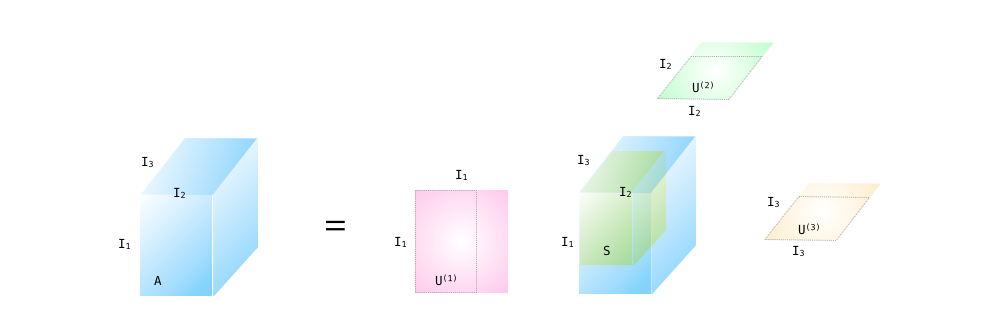
\includegraphics[width=1.00\textwidth]{figures/fig4311.png}
	\caption[The picture of HOSVD for a rank-3 tensor.]{The picture of HOSVD for a rank-3 tensor $A$. $U^{(1)}$,$U^{(2)}$ and $U^{(3)}$ are unitary matrices and $S$ (yellow cuboid) is a core tensor.}
	\label{fig4311}
\end{figure}

According to the theorem of HOSVD \cite{}, every \textit{complex} ($ I_1 \times I_2 \times \dots \times I_N$)-tensor $A$ could be decompose to a \textit{core tensor} $S$ and other $n$-mode unitary matrix $U^{(n)}$, where the maximum of $n$ must be smaller than $N$,
\begin{align}
	A = S \times U^{(1)} \times U^{(2)} \times \dots \times U^{(n)}
\end{align} 
As shown in Fig. \ref{fig4311}, a rank-3 tensor $A$ is decomposed to a core tensor $S$ (yellow cuboid) and three unitary matrices obtaining from three different modes.  The core tensor $S$ is a \textit{complex} ($ I_1 \times I_2 \times \dots \times I_N$)-tensor and have some significant properties, \begin{enumerate}
	\item Row-orthogonal: Two subtensors $S_{\alpha}^{(n)}$ and $S_{\beta}^{(n)}$ are orthogonal when $\alpha \neq \beta$. 
		\begin{align}		
			\left\langle S^{(n)}_{\alpha},S^{(n)}_{\beta} \right\rangle \quad \text{, if} \quad \alpha = \beta
		\end{align}		
		In other words, no matter the shape of $S$, each rows are orthogonal.
	\item Ordering: The Frobenius-norms $\text{ } \norm{S^{(n)}_{i}} $ is ordered from large to small.
		\begin{align}		
			\norm{S^{(n)}_1} \geq \norm{S^{(n)}_2} \geq \dots \geq \norm{S^{(n)}_{I_n}} \geq 0,
		\end{align}		
		for all possible values of $n$.
\end{enumerate}
\begin{figure}[ht]
	\centering
	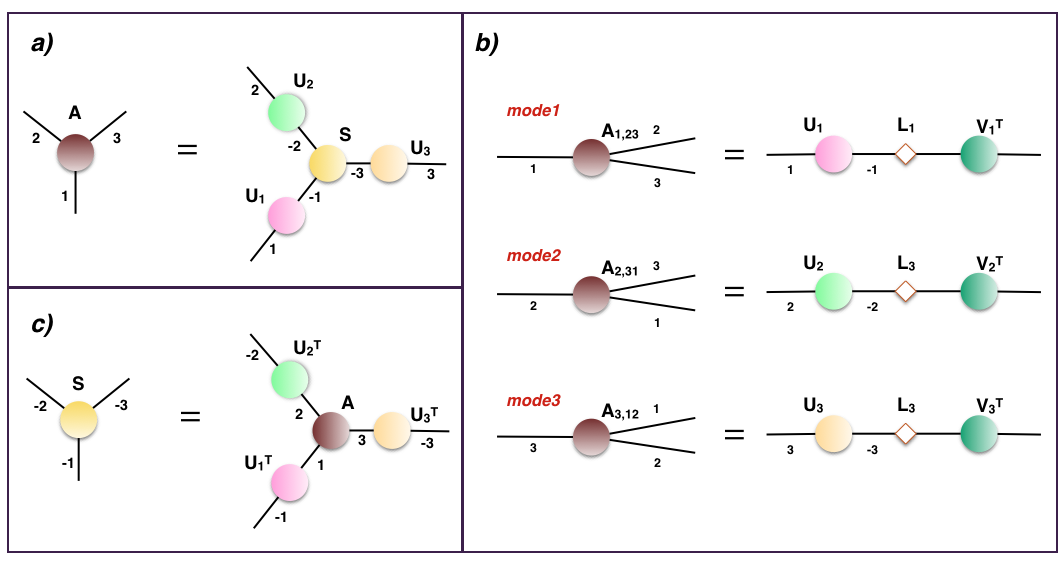
\includegraphics[width=0.90\textwidth]{figures/fig4312.png}
	\caption[The tensor-network representation of HOSVD]{(a) Decompose $A$ to a core tensor $S$ and $n$-mode unitary matrix $U^{(n)}$, (b) Obtain tensors $U^{(n)}$ from decomposing various modes of tensor $A$ by SVD, (c) Obtain the core tensor $S$ from contracting all transpose unitary tensors $U^{(n)T}$ }
	\label{fig4312}
\end{figure}
Now that we show the tensor-network representation for explaining more explicitly. If the target is to decompse a rank-3 $(N=3)$ tensor $A$ by 3 $(n=3)$ modes, see in Fig .\ref{fig4312}(a), we can implement is by the following steps, 
\begin{enumerate}
	\item	Reshaping the tensors to each modes and obtain $U^{(n)}$ by SVD , as shown in Fig. \ref{fig4312}(b).
	\item	Contract all $U^{(n)T}$ tensors for getting $S$ express more mathematically, 
		\begin{align}
			S = A \times U^{(1)T} \times U^{(2)T} \times \dots \times U^{(n)T}
		\end{align} 
		, see Fig. \ref{fig4312}(c).
\end{enumerate}
\subsection{Simple update for PESS}
In chapter.\ref{chapter:2ditebd}, we have introduced an efficient approximation, the "simple update", for determining the PEPS wave function. In principle, the wave function of PESS can be approached by the same way.
In PEPS structure, the ground-state wave function is approximated by iterated application of imaginary-time evolution operators $U(\tau) = e^{-\tau H}$ on an random PEPS state $\Ket{\Psi_t}$, where $\tau$ is a small constant, see Fig. \ref{fig312}. Base on the scheme, we can obtain the ground-state wave function of PESS by following steps,
\begin{enumerate}
	\item Split Hamiltonian $H$,  
		\begin{align}
			\label{splitH}
			H = H_{\alpha} + H_{\beta}
		\end{align}
		where $\alpha$ and $\beta$ are dependent on the geometry of the PESS structure.
	\item Obtain the evolution operator $U(\tau)$ by Trotter-Suzuki decomposition.
		\begin{align}
			e^{-\tau H} = e^{-\tau H_{\alpha}} e^{-\tau H_{\beta}} + O(\tau^{2}).
		\end{align}
	\item Absorb the environment bond vectors, which are considered as the entanglement between each simplex states, into projection tensors, and contract all projection tensors in the simplex state with the core tensor to obtain a cluster tensor.
	\item Apply the evolution operator $U$ to the cluster tensor for obtaining a new cluster tensor.
	\item Decompose the new cluster tensor by HOSVD.
	\item Truncate all the projection tensors and the core tensor.
	\item Absorb the inverse bond vectors for removing the entanglement on the projection tensors.
\end{enumerate}
which is similar to simple update of PEPS. In the following subsections, we applied various cases to explain it more explicitly.
\section{Infinite Kagome lattice}
\label{kagome}
In the previous section, we have briefly introduced to the procedures of PESS ansatz. The first step is to  choose an suitable $n$-PESS structure, where $n$ is the number of projection tensors in a simplex, to split the Hamiltonian and describe the system. There are many various graphical representation for the Kagome lattice [Fig. \ref{fig411}(a)], such as 3-PESS, 5-PESS and 9-PESS, shown in ref. \cite{}. In this section, we will discuss more details about 3-PESS and 5-PESS.
\subsection{3-PESS}
In the 3-PESS case, the PESS state can be drawn as the Fig. \ref{fig4321}(a), which pictures that the many-body states can be described by composing two different simplices, upward- and downward-oriented triangular as shown in Fig \ref{fig4321}(b). Each simplices contain three rank-3 projection tensors, $A^{\sigma_i}_{mm^{\prime}}$ $A^{\sigma_j}_{nn^{\prime}}$ and $A^{\sigma_k}_{ll^{\prime}}$ and a rank-3 core tensor, $S_{mnl}^{\alpha}$ or $S_{m^{\prime}n^{\prime}l^{\prime}}^{\beta}$. Therefore, the form of the Hamiltonian is re-written by eq. \ref{splitH},
\begin{align}
	H = H_{\alpha} + H_{\beta} \quad,\text{where} \quad H_{\alpha} = H_{\Delta},\quad H_{\beta} = H_{\nabla}
\end{align}
Next, utilize the imaginary-time evolution operator $e^{-\tau H}$ to an random initial state $\Ket{\Psi_{0}}$ iteratively. According to the theorem of Trotter-Suzuki decomposition, the evolution operator can be decomposed into two product terms, when $\tau \rightarrow 0$. Hence, the evolution operator operator of 3-PESS can be written as, 
\begin{align}
	\label{eq415}
	e^{-\tau H} = e^{-\tau H_{\Delta}} e^{-\tau H_{\nabla}} + O(\tau^2)
\end{align}
when the value of $\tau$ is small enough. 
\label{3pess}
\begin{figure}[ht]
	\centering
	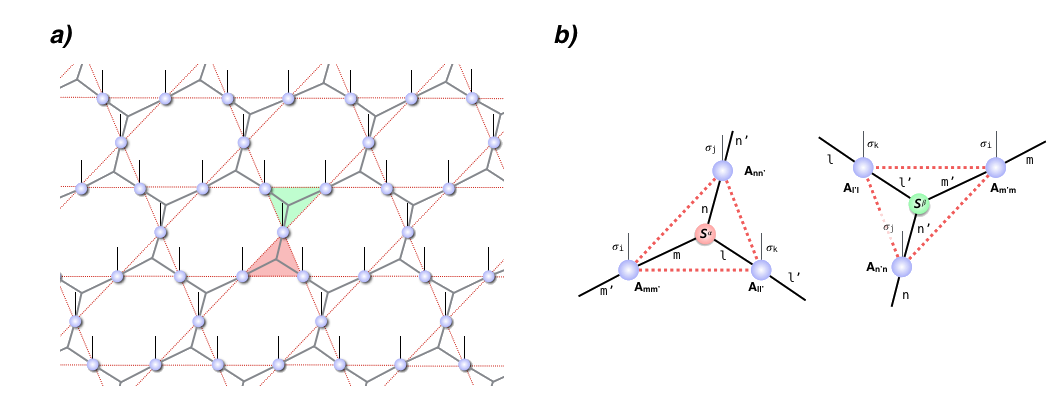
\includegraphics[width=1.00\textwidth]{figures/fig4321.png}
	\caption[The graphical representation of 3-PESS]{The graphical representation of 3-PESS. (a) The PESS state can be considered as composed by two simplices, upward- (green triangular) and downward-triangular (green triangular). The red dash-line represent as the geometry of the kagome lattice. As this figure shown, the projection tensors (Blue circle) are rank-3 with the dimension $dD^2$, where $d$ is the dimension of the physical basis and $D$ is the dimension of the virtual bonds (gray line), and the entangled simplex tensors, with the dimension $D^3$, are located at the cross of three virtual bonds (gray line) in each simplex states. (b) Two simplices in 3-PESS structure. These two type simplices, clustered with the sharing projection tensors, $A^{\sigma_i}_{mm^{\prime}}$, $A^{\sigma_j}_{nn^{\prime}}$ and $A^{\sigma_k}_{ll^{\prime}}$. However, their entangled simplex tensor are individual. In (a), the core tensor of the red simplex is $S^{\alpha}_{mnl}$ and the green one is $S^{\beta}_{m^{\prime}n^{\prime}l^{\prime}}$}
	\label{fig4321}
\end{figure}

After determining the evolution operators, $e^{\tau H_{\Delta}}$ and $e^{\tau H_{\nabla}}$, we apply the schem of the simple update to approximate theground state wave function of 3-PESS. As shown in Fig. \ref{fig4323}, we take an example of updating upward-triangular simplex $\alpha$ to illustrate,

\begin{figure}[ht]
	\centering
	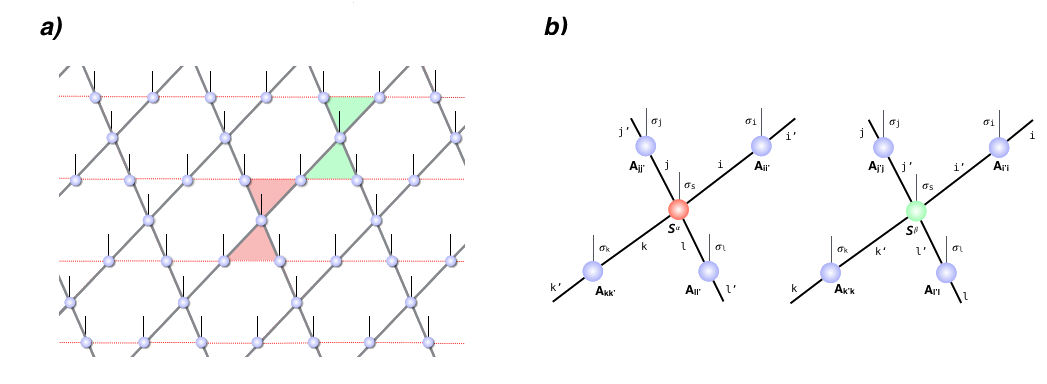
\includegraphics[width=1.00\textwidth]{figures/fig4322.png}
	\caption[The schem of the simple update for 3-PESS.]{The schem of the simple update for 3-PESS. The more detail descriptions are in the paragraph}
	\label{fig4322}
\end{figure}

\begin{enumerate}
	\item Obtain a clustered simplex tensor $\theta$: Firstly, absorb all the environment bond vectors surrounding the simplex state. See Fig. \ref{fig4322}(a),  the environment vectors, $\lambda^{\beta}_{m^{\prime}m}$ , $\lambda^{\beta}_{n^{\prime}n}$ and $\lambda^{\beta}_{l^{\prime}l}$, are obtained from the entangled simplex tensor of simplex $\beta$, due to the canonical form of the PESS \cite{},
		\begin{align}
			&\sum_{n,l}{S^{(\beta)}_{mnl}\left( S^{(\beta)}_{m^{\prime}nl}\right)} = \delta_{m,m^{\prime}} \lambda^{(\beta)^2}_{m} \\
			&\sum_{l,m}{S^{(\beta)}_{mnl}\left( S^{(\beta)}_{mn^{\prime}l}\right)} = \delta_{n,n^{\prime}} \lambda^{(\beta)^2}_{n} \\
			&\sum_{m,n}{S^{(\beta)}_{mnl}\left( S^{(\beta)}_{mnl^{\prime}}\right)} = \delta_{l,l^{\prime}} \lambda^{(\beta)^2}_{l}
		\end{align}
		and base on the features of HOSVD, shown in eq. \ref{}. The $\lambda$s can be simply obtained, when we decompose the clustered tensors of the simplex $\beta$ in the updating process. Secondly, contract all tensors in simplex state to obtain the clustered tensor $\theta$. The mathematical representation of the step is written as,  
		\begin{align}
			\theta_{m^{\prime} n^{\prime} l^{\prime}}^{\sigma_i \sigma_j \sigma_k} = \sum_{mnl,m^{\prime}n^{\prime}l^{\prime}}{S^{(\alpha)}_{mnl} \lambda^{(\beta)}_{m^{\prime \prime}} A^{\sigma_i}_{mm^{\prime}} \lambda^{(\beta)}_{n^{\prime \prime}} A^{\sigma_j}_{nn^{\prime}} \lambda^{(\beta)}_{l^{\prime \prime}} A^{\sigma_k}_{ll^{\prime}}}
		\end{align}
	\item Apply the evolution operator $U(\tau)$: In eq. \ref{eq415}, we have generated the evolution operator for 3-PESS ansatz. Due to updating upward-triangles simplex, $U(\tau)$ is defined as, 
		\begin{align}
			U(\tau) = e^{-\tau H_{\Delta}}
		\end{align}
		Now that, we utilize $U(\tau)$ to the cluster tensor $\theta$, see Fig. \ref{fig4322}(c) and obtain a new cluster tensor $\theta^{\prime}$, 
	\item Decompose $\theta^{\prime}$ into the general form of the simplex state: Apply the high-order singular value decomposition (HOSVD) to obtain new projection tensors, $U^{(\sigma_i)}$, $U^{(\sigma_j)}$ and $U^{(\sigma_k)}$, and a new core tensor of simplex $\alpha$, $S^{(\alpha)^{\prime}}$, see Fig. \ref{fig4322}(d). During operating HOSVD, we need save the environment bond vectors, $\lambda^{(\alpha)}_{m}$, $\lambda^{(\alpha)}_{n}$ and $\lambda^{(\alpha)}_{l}$, surrounding the simplex $\beta$. All $\lambda^{(\alpha)}$ could be obtained from decomposing different modes of $\theta^{\prime}$. As shown in Fig. \ref{fig4312}(b).
	\item Truncation: In order to avoid the exponential increment of the virtual bonds dimension, we need truncate the brown bonds in Fig. \ref{fig4322}(d) to specified dimension $D^{\prime}$ which can be fixed to original dimension $D$ or determined dynamically by setting an truncation error as the discussion in section \ref{truncationerror}. The simple way is to truncate projection tensors firstly,  
		\begin{align}
			&U^{\sigma_i} \rightarrow \widetilde{U}^{\sigma_i}_{mm^{\prime}} \\
			&U^{\sigma_j} \rightarrow \widetilde{U}^{\sigma_j}_{nn^{\prime}} \\
			&U^{\sigma_k} \rightarrow \widetilde{U}^{\sigma_k}_{ll^{\prime}}
		\end{align}
		Next, contract the transpose of these tensors with $\theta^{\prime}$, as Fig. \ref{fig4312}(c), to obtain $\widetilde{S}^{\alpha}$ in Fig. \ref{fig4322}(e), where
		\begin{align}
			\widetilde{S}^{(\alpha)} = \sum_{m^{\prime}n^{\prime}l^{\prime}}{\theta_{m^{\prime} n^{\prime} l^{\prime}}^{\prime \sigma_i \sigma_j \sigma_k} \widetilde{U}^{\sigma_i}_{mm^{\prime}} \widetilde{U}^{\sigma_j}_{nn^{\prime}} \widetilde{U}^{\sigma_k}_{ll^{\prime}}}
		\end{align}
	\item Absorb the inverse environment bond vectors $\lambda^{(\beta)^{-1}}$ into truncated projection tensors: To obtain the updated projection tensors $\widetilde{A}^{\sigma_i}_{mm^{\prime}}$, $\widetilde{A}^{\sigma_j}_{nn^{\prime}}$ and $\widetilde{A}^{\sigma_k}_{ll^{\prime}}$, we need remove the influence of environment, 
		\begin{align}
			\widetilde{A}^{\sigma_i}_{mm^{\prime}} &= \sum_{m^{\prime \prime}}{ \lambda^{(\beta)}_{m^{\prime} m^{\prime \prime}} \widetilde{U}^{\sigma_i}_{mm^{\prime \prime}}} \\
			\widetilde{A}^{\sigma_j}_{nn^{\prime}} &= \sum_{n^{\prime \prime}}{ \lambda^{(\beta)}_{n^{\prime} n^{\prime \prime}} \widetilde{U}^{\sigma_j}_{nn^{\prime \prime}}} \\
			\widetilde{A}^{\sigma_k}_{ll^{\prime}} &= \sum_{l^{\prime \prime}}{ \lambda^{(\beta)}_{l^{\prime} l^{\prime \prime}} \widetilde{U}^{\sigma_i}_{ll^{\prime \prime}}}
		\end{align}	
		see Fig. \ref{fig4322}(f),
\end{enumerate}

At here, one updated epoch is completed. Finally, the ground state will be obtained by iterating the procedures for each simplex, upward- and downward- triangular $(\Delta, \nabla)$, until the wave function of PESS converge, 
%$\mathlarger{\rjoin}$
\subsection{5-PESS}
In the 5-PESS structure [Fig. \ref{fig4323}(a)], the procedure to approximate the ground state wave function is similar to 3-PESS. However, due to the transformation of the structure, the simplices should be re-defined. In the 5-PESS ansatz, each simplex state is composed by an upward- and a downward-triangular and the most significant change is that the core tensors are located on the physical sites. As shown in Fig. \ref{fig4323}(b), each simpliices contain 4 projection tensors $A^{\sigma_i}_{ii^{\prime}}$ $A^{\sigma_j}_{jj^{\prime}}$ $A^{\sigma_k}_{kk^{\prime}}$ and $A^{\sigma_l}_{ll^{\prime}}$, and a core tensor, $S^{\sigma_s (\alpha)}_{ijkl}$ or $S^{\sigma_s (\beta)}_{i^{\prime}j^{\prime}k^{\prime}l^{\prime}}$. Therefor, we can split the Hamiltonian into 
\begin{align}
	H = H_{\alpha} + H_{\beta} \quad \text{,where} \quad H_{\alpha} = H_{\rjoinr}, H_{\beta} = H_{\rjoing}
\end{align}
and as previous section, the evolution operator is written as, 
\begin{align}
	e^{-\tau H} = e^{-\tau H_{\rjoinr}} e^{-\tau H_{\rjoing}} + O(\tau^2)
\end{align}
when $\tau \rightarrow 0$.

\label{5pess}
\begin{figure}[ht]
	\centering
	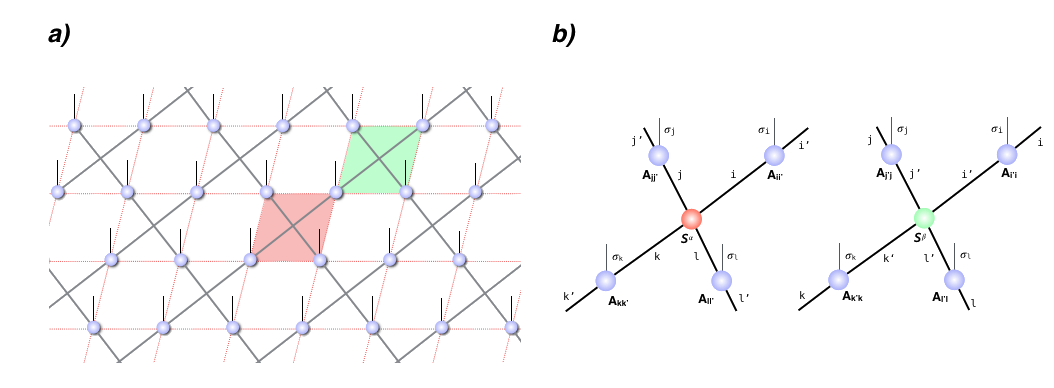
\includegraphics[width=1.00\textwidth]{figures/fig4323.png}
	\caption[The graphical representation of 3-PESS]{The graphical representation of 3-PESS. (a) The PESS state can be considered as composed by two simplices, upward- (green triangular) and downward-triangular (green triangular). The red dash-line represent as the geometry of the kagome lattice. As this figure shown, the projection tensors (Blue circle) are rank-3 with the dimension $dD^2$, where $d$ is the dimension of the physicla basis and $D$ is the dimension of the virtual bonds (gray line), and the entangled simplex tensors, with the dimension $D^3$, are located at the cross of three virtual bonds (gray line) in each simplex states. (b) Two simplices in 3-PESS structure. These two type simplices, clustered with the sharing projection tensors, $A^{\sigma_i}_{mm^{\prime}}$, $A^{\sigma_j}_{nn^{\prime}}$ and $A^{\sigma_k}_{ll^{\prime}}$. However, their entangled simplex tensor are individual. In (a), the core tensor of the red simplex is $S^{\alpha}_{mnl}$ and the green one is $S^{\beta}_{m^{\prime}n^{\prime}l^{\prime}}$}
	\label{fig4323}
\end{figure}
Next, apply the simple update scheme as Fig. \ref{fig4324}. Most of steps are similar to 3-PESS, shown as Fig. \ref{fig4322}. However, we should carefully decompose the cluster tensor $\theta^{\prime}$, where
\begin{align}
	\theta^{\prime} = \theta \times U(\tau)
\end{align}
see Fig. \ref{fig4324}(d). In this structure, the core tensors contain physical basis states, which means that it can't be decompose by the simply way shown in Fig. \ref{fig4312}, due to
\begin{align}
	N \mod n \neq 0
\end{align}
where $N$ is the rank of the tensor $\theta^{\prime}$ and $n$ is the mode number of HOSVD. Hence, the bond $\sigma_s$, belonging to the core tensor $S^{(\alpha)}_{i^{\prime}j^{\prime}k^{\prime}l^{\prime}}$ in tensor $\theta^{\prime}$, must be fixed during the decomposition. The more detail and general form of the HOSVD are written in the documentation of \textit{Uni10 Library} \cite{}, which is implemented by c/c++ and helpful for calculating the high-rank linear algebra problems.
\begin{figure}[ht]
	\centering
	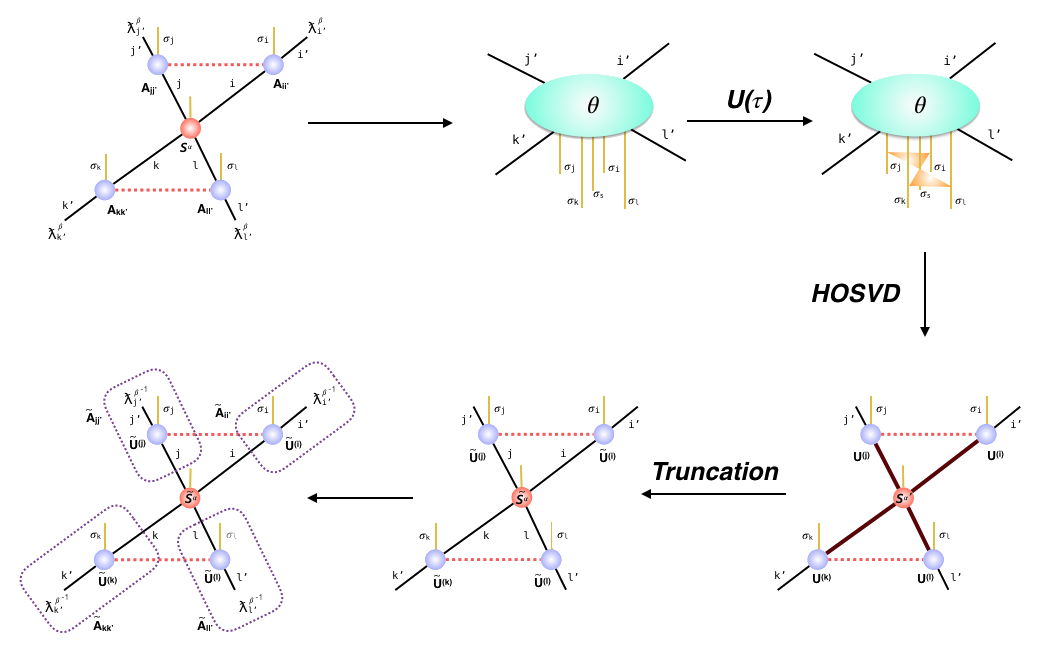
\includegraphics[width=1.00\textwidth]{figures/fig4324.png}
	\caption[The schem of the simple update for 5-PESS.]{The schem of the simple update for 5-PESS. The more detail descriptions are in the paragraph}
	\label{fig4324}
\end{figure}
\section{Infinite Square lattice}
\label{4pess2b}
In previous sec. \ref{kagome}, we have verified the results in ref. \cite{} \cite{}. In order to test and recognize the properties of the PESS ansatz more explicitly, we extend it to simulate infinite square systems and compare it with methods discussed in chap. \ref{chapter:2ditebd}.
\subsection{4-PESS (Rank-3 projection tensors)}
The 4-PESS structure could be build by two different methods, which is drawn in the ref. \cite{}. In this section, we use the concept, shown in Fig. \ref{fig4325}(a), to complete the implementation. 

See Fig. \ref{fig4325}(a), the many-body state can be regarded as composed by two different simplices, shown in Fig. \ref{fig4325}(b), repeatedly. The components of each simplices are similar to 5-PESS, but the difference is that the core tensors, $S^{(\alpha_)}_{ijkl}$ and $S^{(\beta)}_{i^{\prime}j^{\prime}k^{\prime}l^{\prime}}$, are not located on the lattice sites. Hence, the Hamiltonian is split into,
\begin{align}
	H = H_{\alpha} + H_{\beta} \quad,\text{where} \quad H_{\alpha} = H_{\color{red} \square},\quad H_{\beta} = H_{\color{green} \square}
\end{align}
where ${\color{red} \square}$ and ${\color{green} \square}$ are represented simplex $\alpha$ and $\beta$, shown in Fig. \ref{fig4325}(b). Therefor, the evolution operator can be written as, 
\begin{align}
	e^{-\tau H} = e^{-\tau H_{\color{red} \square}} e^{-\tau H_{ \color{green} \square}} + O(\tau^2)
\end{align}
when $\tau$ is a small constant $\rightarrow 0$.
\begin{figure}[ht]
	\centering
	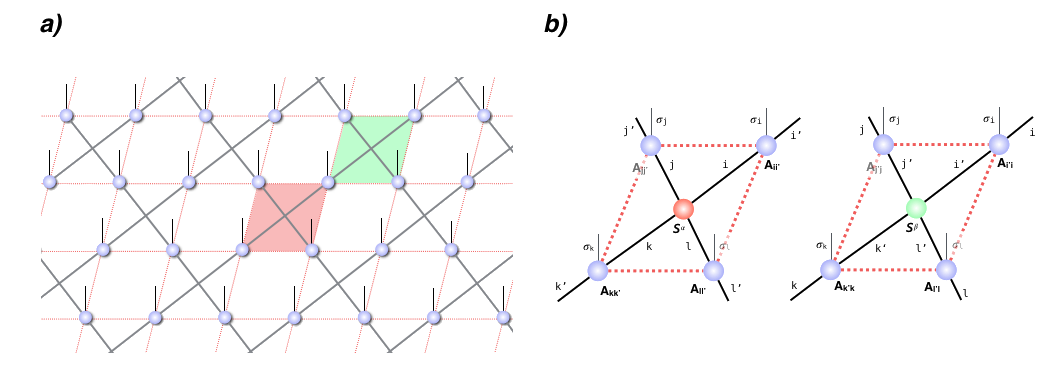
\includegraphics[width=1.00\textwidth]{figures/fig4325.png}
	\caption[The graphical representation of 3-PESS]{The graphical representation of 3-PESS. (a) The PESS state can be considered as composed by two simplices, upward- (green triangular) and downward-triangular (green triangular). The red dash-line represent as the geometry of the kagome lattice. As this figure shown, the projection tensors (Blue circle) are rank-3 with the dimension $dD^2$, where $d$ is the dimension of the physicla basis and $D$ is the dimension of the virtual bonds (gray line), and the entangled simplex tensors, with the dimension $D^3$, are located at the cross of three virtual bonds (gray line) in each simplex states. (b) Two simplices in 3-PESS structure. These two type simplices, clustered with the sharing projection tensors, $A^{\sigma_i}_{mm^{\prime}}$, $A^{\sigma_j}_{nn^{\prime}}$ and $A^{\sigma_k}_{ll^{\prime}}$. However, their entangled simplex tensor are individual. In (a), the core tensor of the red simplex is $S^{\alpha}_{mnl}$ and the green one is $S^{\beta}_{m^{\prime}n^{\prime}l^{\prime}}$}
	\label{fig4325}
\end{figure}

Finally, the ground state wave function can be obtained by repeating the following steps, shown in Fig. \ref{fig4326}, on the simplices, $\alpha$ and $\beta$ $( \color{red} \square$, ${\color{green} \square})$, until the wave function of PESS converge.

Before we do more restrict comparisons, it is obvious that the control of dimensional increment in the 4-PESS is better than in the PEPS [Fig. \ref{fig314}], In 4-PESS structure, the projection tensors are described by rank-3 tensors whose dimension is $dD^2$. However, in the PEPS representation, the dimension of local tensors is $dD^4$. The reduction of tensors dimension is helpful for calculating and studying with a significant larger dimension. Nevertheless, it doesn't also mean that the 4-PESS algorithm is more efficient than PEPS one and actually it encounter in some problems when approximating the environment. We will show mare details in following sections.

\begin{figure}[ht]
	\centering
	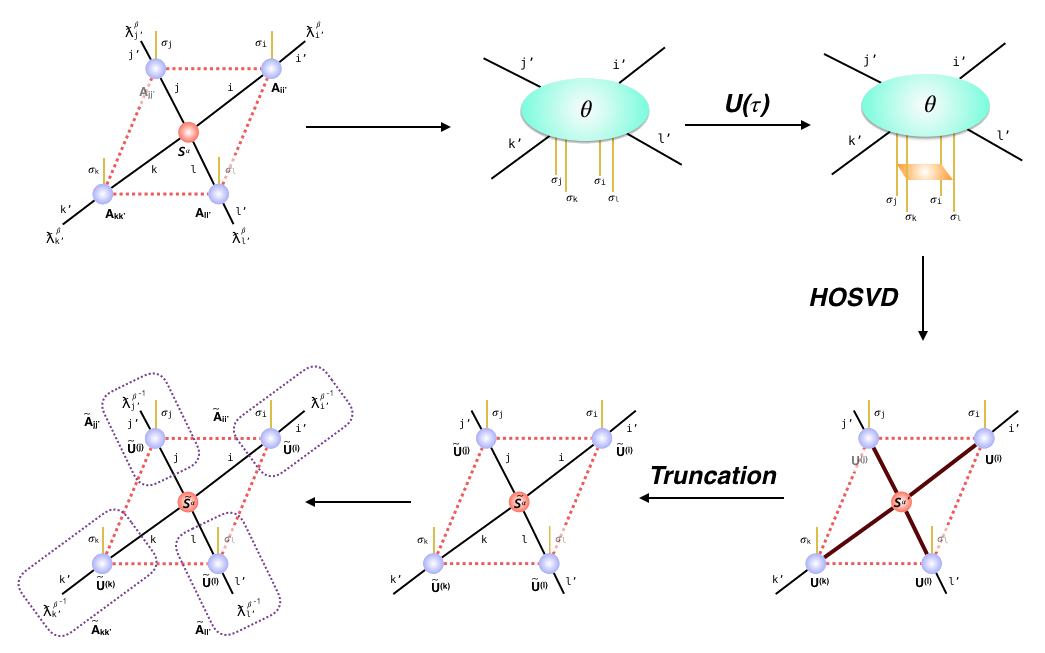
\includegraphics[width=1.00\textwidth]{figures/fig4326.png}
	\caption[The scheme of the simple update for 4-PESS, composed by rank-3 projection tensors.]{The scheme of the simple update for 4-PESS, composed by rank-3 projection tensors. The more detail descriptions are in the paragraph}
	\label{fig4326}
\end{figure}

\section{Properties of PESS algorithm}

\subsection{3PESS on infinite Kagome lattice}

Before applying the PESS algorithms to study square lattice systems, we should know and verify some features. At beginning, we present the results for the Heisenberg model on Husimi lattice \cite{},

\subsubsection{$S=1$}

In the $S=1$ Heisenberg model on the Husimi lattice, the ground state energy per sites $E_0$ decrease with virtual dimension $D$ and converge to $E_0=-1.405$ rapidly, see Fig.\ref{fig4327}. However, according to the theory of the simplex solid states [Sec. \ref{solidstate}], a physical $S=2n-1$ spin can be regarded as a symmetric superposition of a virtual $S=n-1$ and a virtual $S=n$ spin. We predict that there are two different ground state energy between the two simplices (upward- and downward-triangular). As shown in Fig. \ref{fig4328}, the energy difference
\begin{align}
	\Delta E = 2 \frac{|E_{\Delta}-E_{\nabla}|}{3}
\end{align}
and the spontaneous magnetization
\begin{align}
	M = \frac{1}{N} \sum_{i}{\sqrt{\braket{S_x}^2 + \braket{S_y}^2 + \braket{S_z}^2}}
\end{align}
can be considered as two different order parameters. The energy difference $\Delta E$ rapid increase to a constant value and the magnetic order parameter $M$ begin to rapid fall to zero almost at the same time, where $D=8$. It means that to describe the simplices states, the requirement of virtual bond dimension $D_c$ must be larger than $8$. The results is also corresponds to the theory of the simplex solid states.

\begin{figure}[H]
	\centering
	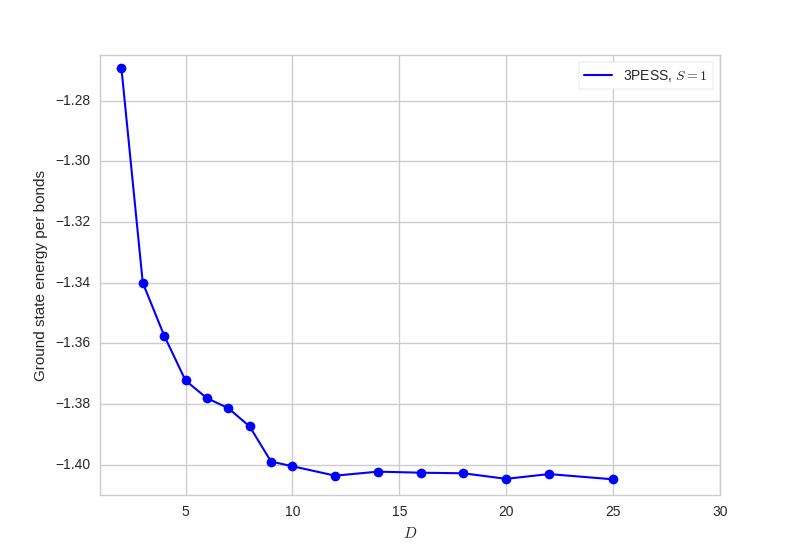
\includegraphics[width=0.75\textwidth]{figures/3pess_S1GE.png}
	\caption[The scheme of the simple update for 4-PESS, composed by rank-3 projection tensors.]{The scheme of the simple update for 4-PESS, composed by rank-3 projection tensors. The more detail descriptions are in the paragraph}
	\label{fig4327}
\end{figure}

\begin{figure}[ht]
	\centering
	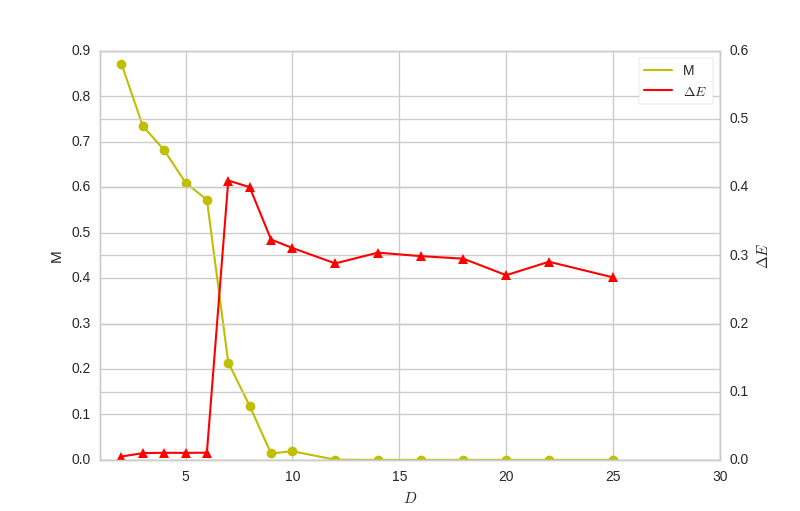
\includegraphics[width=0.80\textwidth]{figures/3pess_MDE.png}
	\caption[The scheme of the simple update for 4-PESS, composed by rank-3 projection tensors.]{The scheme of the simple update for 4-PESS, composed by rank-3 projection tensors. The more detail descriptions are in the paragraph}
	\label{fig4328}
\end{figure}

\begin{figure}[ht]
	\centering
	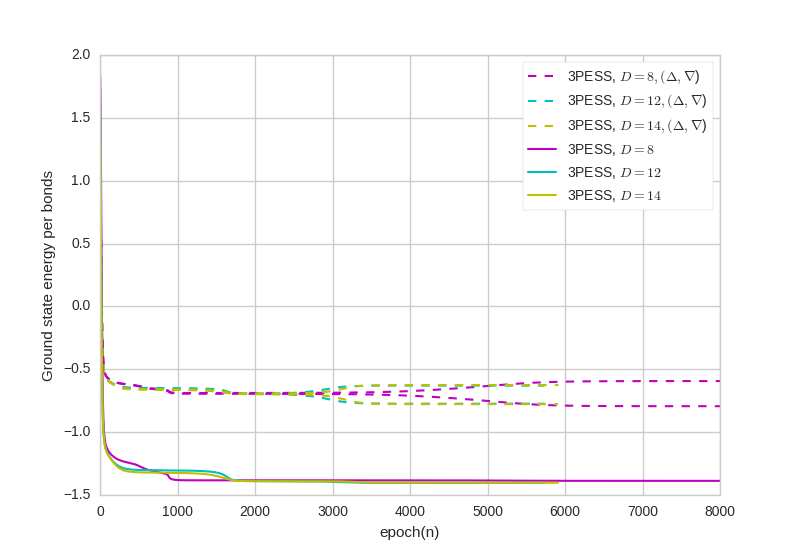
\includegraphics[width=0.80\textwidth]{figures/3pess_GEN.png}
	\caption[The scheme of the simple update for 4-PESS, composed by rank-3 projection tensors.]{The scheme of the simple update for 4-PESS, composed by rank-3 projection tensors. The more detail descriptions are in the paragraph}
	\label{fig4329}
\end{figure}

\subsubsection{$S=2$}

\begin{figure}[ht]
	\centering
	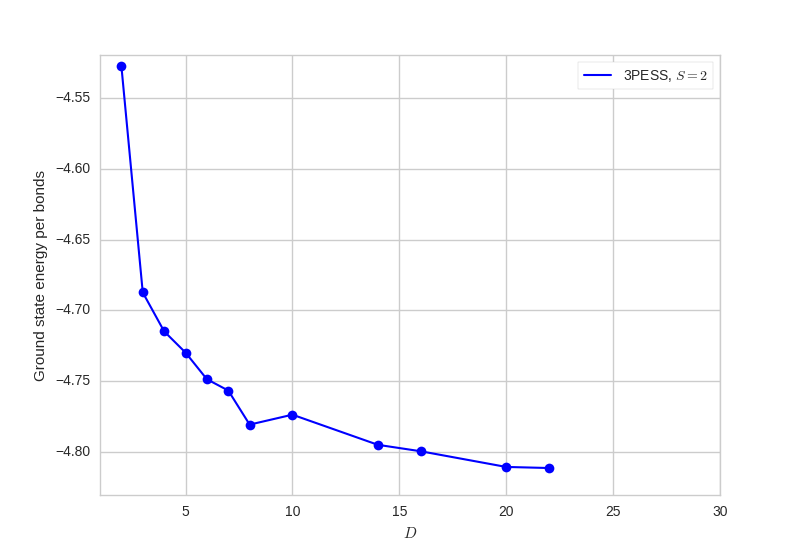
\includegraphics[width=0.80\textwidth]{figures/3pess_S2GE.png}
	\caption[The scheme of the simple update for 4-PESS, composed by rank-3 projection tensors.]{The scheme of the simple update for 4-PESS, composed by rank-3 projection tensors. The more detail descriptions are in the paragraph}
	\label{fig4330}
\end{figure}

\begin{figure}[!ht]
	\centering
	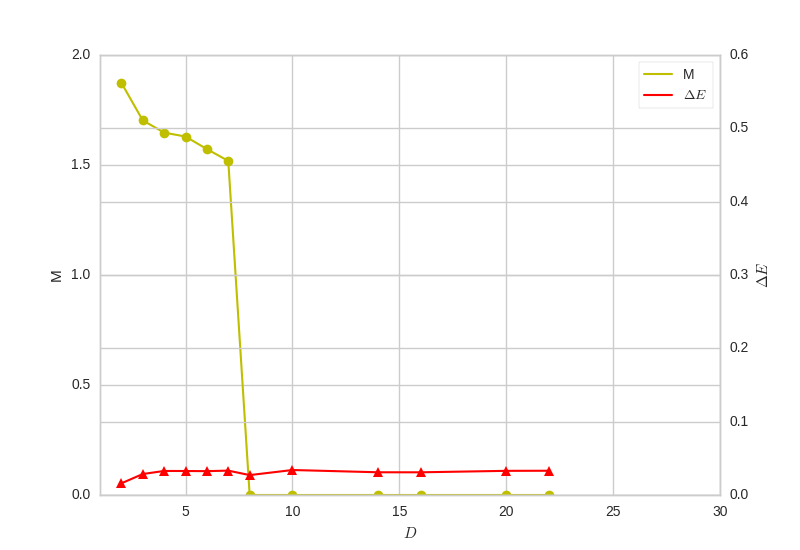
\includegraphics[width=0.80\textwidth]{figures/3pess_S2M.png}
	\caption[The scheme of the simple update for 4-PESS, composed by rank-3 projection tensors.]{The scheme of the simple update for 4-PESS, composed by rank-3 projection tensors. The more detail descriptions are in the paragraph}
	\label{fig4330}
\end{figure}

\subsection{4PESS for Heisenberg model on square lattice}

\begin{figure}[ht]
	\centering
	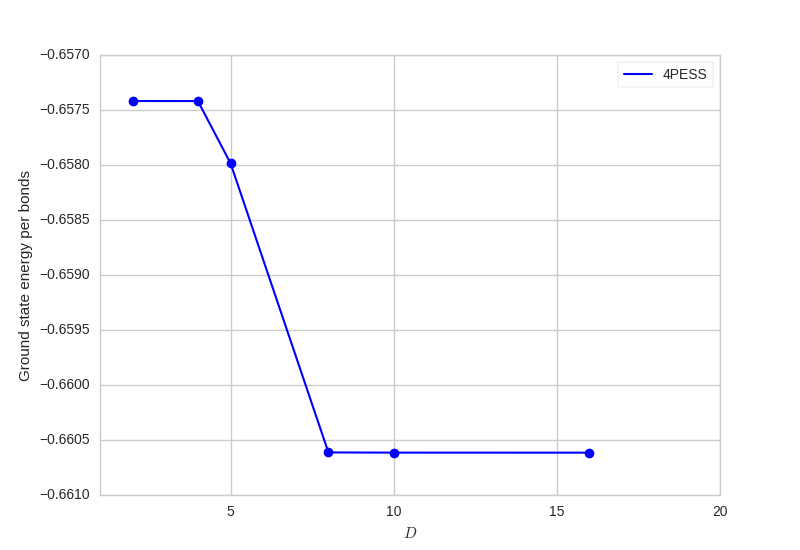
\includegraphics[width=0.80\textwidth]{figures/4pess_HeiGE.png}
	\caption[The scheme of the simple update for 4-PESS, composed by rank-3 projection tensors.]{The scheme of the simple update for 4-PESS, composed by rank-3 projection tensors. The more detail descriptions are in the paragraph}
	\label{fig4331}
\end{figure}

\subsection{Comparison between PESS and iPEPS}

